\chapter{Motivazione e basi}


\section{Mappa di Poincar\'e}
Proviamo a capire quando un sistema di equazioni differenziali porta un'orbita a tornare vicino a se stessa.

\begin{definition}[Mappa di Poincar\'e]
Sia $M$ una variet\`a e sia $\Sigma$ una sua sottovariet\`a di codimensione 1 tale che esiste $U\subseteq \Sigma$ con la seguente propriet\`a:\\
se $P\in U$ allora esiste $\ol t>0$ tale che $t\in (0,\ol t)\implies \phi_t(P)\notin U$ e $\phi_{\ol t}(P)\in U$\footnote{$\ol t$ \`e l'istante del ``primo ritorno"}.\\
Definiamo la \textbf{mappa di Poincar\'e} come
\[P_U:\funcDef{U}{U}{(x,y)}{\phi_{\ol t}(x,y)}.\]
\end{definition}
\begin{remark}
Se $P_\Sigma^n=\under{n\text{ volte}}{P_\Sigma\circ\cdots\circ P_\Sigma}$, ponendo $P_\Sigma^0=id$ stiamo definendo un sistema discreto $(\Sigma,P_\Sigma,\Z)$\footnote{$P_\Sigma^{-1}$ \`e definita perch\'e sono partito da un flusso e posso prendere tempi negativi in un flusso}.
\end{remark}

\begin{example}[Moto sul toro piatto]
Sia $T^2=\R^2/\Z^2$. Un moto geodetico sul toro (piatto) si pu\`o pensare come
\[t\mapsto \phi_t(x,y)=(x,y)+t(v_x,v_y)\mod{\Z^2}.\]
Sia $\Sigma=U=S^1=\quot{[0,1]\times\cpa0}{(0,0)\sim(1,0)}$. Per la geometria del toro questa sottovariet\`a di $T^2$ ha le propriet\`a richieste per definire la mappa di Poincar\'e (addirittura sappiamo che $\ol t=1/v_y$).\\
Esplicitamente troviamo che 
\[P_\Sigma:\funcDef{S^1}{S^1}{t}{t+\al \mod 1}\]
dove $\al=v_x/v_y$. Osserviamo che a meno di traslare modulo 1, tutte le orbite sono determinate dall'orbita di $0$.
\setlength{\leftmargini}{0cm}
\begin{itemize}
\item[$\boxed{\al\in\Q}$] Se $\al=\frac pq$ ridotta ai minimi termini allora $P_\Sigma^q(0)=0+p=0 \mod 1$ e le orbite sono periodiche.
\item[$\boxed{\al\in\R\bs\Q}$] Evidentemente non troviamo un'orbita periodica. \`E possibile mostrare che in realt\`a l'orbita \`e densa.
\end{itemize}
\setlength{\leftmargini}{0.5cm}
\end{example}


\begin{definition}[Semipiano di Poincar\'e]
Consideriamo la regione $[-1,1]\times [0,+\infty]\bs D^1$ e identifichiamo i lati come in figura
\begin{figure}[!htb]
    \centering
    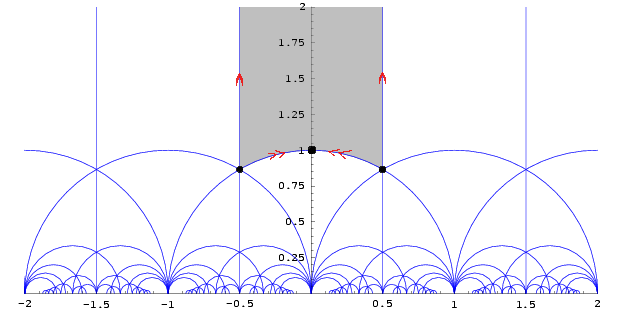
\includegraphics[width=9cm]{Immagini/ModularGroup-FundamentalDomain-01.png}
    \caption{Dominio fondamentale e qualche geodetica.}
    \label{SemipianoPoincare}
\end{figure}

\noindent
Le geodetiche sono le intersezioni dell'oggetto con rette verticali o semicirconferenze perpendicolari all'asse $x$.
Chiamiamo $\Mc$ questo spazio.
\end{definition}
\begin{example}[Geodetiche sul piano di Poincar\'e]
A parte le geodetiche corrispondenti a rette verticali, ogni geodetica che incontra la regione lo fa passando per l'asse $y$ (e quindi lo fa ad un certo angolo). Possiamo associare ad ogni coppia punto di $\Mc$ e angolo una geodetica di $\Mc$ (quella passante per il punto che incontra la verticale a quell'angolo)
\[\Mc\times S^1\ni ((x,y),\theta)\mapsto g_t((x,y),\theta).\]
Sia $\Sigma=\cpa{x=0,y>1}\times S^1$. \`E possibile definire $P_\Sigma$ e si da il caso che questa mappa di Poincar\'e \`e pi\`u facile da studiare rispetto al sistema originale.
\end{example}

\section{Esempi di sistemi discreti caotici}
\begin{example}[Perdo il controllo]
Consideriamo la mappa
\[T:\funcDef{S^1}{S^1}{x}{10x \mod 1}.\]
Poniamo $\Ac=\cpa{0,\cdots,9}$ e $\Ac_n=\pa{\frac n{10},\frac{n+1}{10}}$ per $n\in\Ac$.\\
Sia $x\in \R\bs \Q$ e diamo la seguente mappa
\[\vp:x\mapsto(\omega_0,\omega_1,\cdots)\in \Ac^{\N}\]
dove $\omega_n=k\coimplies T^n(x)\in \Ac_k\coimplies \lfloor10 T^n(x)\rfloor=k$ e per ricorsione vediamo che $\omega_n$ \`e la $n$-esima cifra decimale di $x$, cio\`e
\[x=0.\omega_0\omega_1\omega_2\cdots.\]
Per rispondere ad una domanda del tipo ``$T^{1000}(x)\in \Ac_i?$" devo sapere la 1000-esima cifra di $x$. Se ora considero $x+\e$ al posto di $x$, le informazioni che avevamo su $x$ non dicono pi\`u nulla sul comportamento di $x+\e$ oltre un certo passo\footnote{se $i>-\log_{10} \e$ la risposta a ``$T^{1000}(x)\in \Ac_i?$" e quella a ``$T^{1000}(x+\e)\in \Ac_i?$" sono indipendenti.}.
\end{example}

\begin{remark}[Piccola parentesi statistica]
Sia $x=0.x_1x_2\cdots$ potremmo chiederci, fissata una cifra $k$ se
\[Prob\cpa{\lim_{N\to+\infty}\frac{\#\cpa{i\in \cpa{0,\cdots, N-1}\mid x_i=k}}{N}=\frac1{10}}=1\]
ed effettivamente \`e vero. Segue dunque che
\[Prob\cpa{\lim_{N\to+\infty}\frac{\#\cpa{i\in \cpa{0,\cdots, N-1}\mid x_i=k}}{N}=\frac1{9}}=0\]
anche se non \`e un insieme vuoto\footnote{per esempio posso fissare ogni nona cifra a $k$ e completare le altre con cifre a caso diverse da $k$.}.
\end{remark}

\begin{example}[Oscillatore armonico perturbato]
Sia $f:\R\to \R$ una funzione $1$-periodica. Immaginiamo una palla che rimbalza su un piatto la cui altezza varia come $f$. Per semplificarci la vita possiamo immaginare che l'urto avvenga sempre in $x=0$, tanto l'unica cosa che conta \`e $\dot f$ (l'impulso). Siano $t_0,t_1,\cdots,t_n$ i tempi di urto ($t_0=0$) e siano $v_0,\cdots,v_n$ le velocit\`a dopo l'urto. Conoscendo questi dati possiamo ricostruire tutta la dinamica.
\[T:\funcDef{[0,+\infty)\times (0,+\infty)}{[0,+\infty)\times (0,+\infty)}{(t_{n},v_n)}{(t_{n+1},v_{n+1})}.\]
Calcoliamo
\[\begin{cases}
t_{n+1}=t_n+h(v_n)\\
v_{n+1}=v_n+2\dot f(t_{n+1})
\end{cases},\quad h(v_n)=\frac 2gv_n\]
Osserviamo inoltre che
\[T(t_n+1,v_n)=(t_n+1+h(v_n), v_n+2\dot f(t_n+1 h(v_{n+1})))=T(t_n,v_n)+(1,0),\]
quindi in realt\`a possiamo considerare $S^1$ al posto di $[0,+\infty)$ per i tempi.\\
Questo sistema \`e difficile da trattare e presenta molti problemi aperti.
\end{example}